%!TEX TS-program = xelatex
%!TEX encoding = UTF-8 Unicode
%!TEX root = ../../../LSSN.tex

%------------------------- IMMAGINE TIKZ
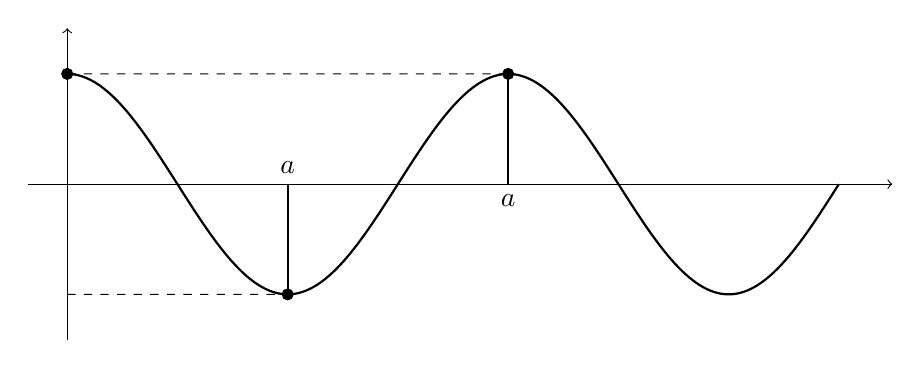
\begin{tikzpicture}[scale=.99]
  \draw[->] (1.414,-2) -- (1.414,2);
  \draw[->] (0.914,0) -- (12,0);
       \coordinate (origin) at (0:0);
       \coordinate (A) at (45:2);
       \coordinate (B) at (-45:2);
       \coordinate (0) at (0:2);
       \coordinate (1) at (7.071,1.414);
       \coordinate (-1) at (4.242,-1.414);
  \filldraw (A) circle (2pt) node[above right] {};
  \draw[dashed] (B) -- (-1);
  \draw[dashed] (A) -- (1);
  \filldraw (1) circle (2pt) node[above] {};
  \filldraw (-1) circle (2pt) node[below] {};

  \draw[thick] (1.414,1.414) cos (2.828,0) sin (4.242,-1.414) cos (5.656, 0) sin (7.071,1.414) cos (8.485,0) sin (9.899,-1.414) cos (11.313,0);

  \draw[thick] (4.242,-1.414) -- (4.242,0) node[above] {$a$};
  \draw[thick] (7.071,1.414) -- (7.071,0) node[below] {$a$};
\end{tikzpicture}
%------------------------- IMMAGINE TIKZ
